%----------------------------------------------------------------------------------------
%	PACKAGES AND THEMES
%----------------------------------------------------------------------------------------
\documentclass[aspectratio=128,xcolor=dvipsnames, notes]{beamer}
\usetheme{SimplePlus}
\usepackage{tikz} % for figures
\usepackage[style=authoryear, bibencoding=utf8, minnames=1, maxnames=3,
maxbibnames=99, natbib=true, dashed=false, terseinits=true,
firstinits=true, uniquename=false, uniquelist=true, labeldate=true,
doi=false, isbn=false, natbib=true, backend=biber, note=false, url=false, eprint=false]{biblatex}
\AtEveryBibitem{\clearlist{language}}
\AtEveryBibitem{%
  \clearfield{note}%
}
\usepackage{dsfont} % for fancy R
\addbibresource{references.bib} 
\usepackage{hyperref}
\usepackage{ragged2e}
\usepackage{enumerate}% http://ctan.org/pkg/enumerate
\usepackage{xcolor}
\usepackage{graphicx} % Allows including images
\usepackage{booktabs} % Allows the use of \toprule, \midrule and \bottomrule in tables

\setbeamertemplate{footline}[frame number]{}
\renewcommand*{\bibfont}{\scriptsize}
\newcommand{\highlight}[1]{%
  \colorbox{yellow!50}{$\displaystyle#1$}}
  \newcommand{\fundmat}{\mathbf{\Phi}(t, 0)}
\newcommand{\fundmats}{\mathbf{\Phi}(t, s)}
\newcommand{\fundmatso}{\mathbf{\Phi}(s, 0)}
\newcommand{\fundmatsu}{\mathbf{\Phi}(s, u)}
\newcommand{\fundmattv}{\mathbf{\Phi}(t, v)}
\newcommand{\Expec}{\mathbb{E}}
\newcommand{\Cov}{\operatorname{Cov}}
%----------------------------------------------------------------------------------------
%	TITLE PAGE
%----------------------------------------------------------------------------------------

\title[short title]{Functional Regression Models in Human Movement Biomechanics} % The short title appears at the bottom of every slide, the full title is only on the title page
\subtitle{Methodology and Applications}

\author[Edward Gunning] {Edward Gunning}

% \institute[NTU] % Your institution as it will appear on the bottom of every slide, may be shorthand to save space
% {
%     Department of Mathematics and Statistics \\
%     University of Limerick % Your institution for the title page
% }
\date{
    \vskip1em
    JHU Biostatistics Wearable and Implantable Technology Group \\
    \vskip1em
    September $13$th $2024$
} % Date, can be changed to a custom date


%----------------------------------------------------------------------------------------
%	PRESENTATION SLIDES
%----------------------------------------------------------------------------------------

\begin{document}

\begin{frame}
    % Print the title page as the first slide
    \titlepage
\end{frame}

\section{Introduction}

\begin{frame}{Background}
\textcite{winter_biomechanics_1979} defines \textbf{human movement biomechanics} as
    \begin{quote}
        ``\dots the inter-discipline that describes, analyses, and assesses human movement" 
    \end{quote}

\begin{itemize}
    \pause \item Data collected on displacement, velocity and acceleration (\textbf{kinematics}) and forces (\textbf{kinetics}).
    \pause \item Continuously measured throughout a movement $\rightarrow$ smooth time-varying curves, very suitable for FDA.
\end{itemize}
\vfill
\pause \begin{figure}
    \centering
    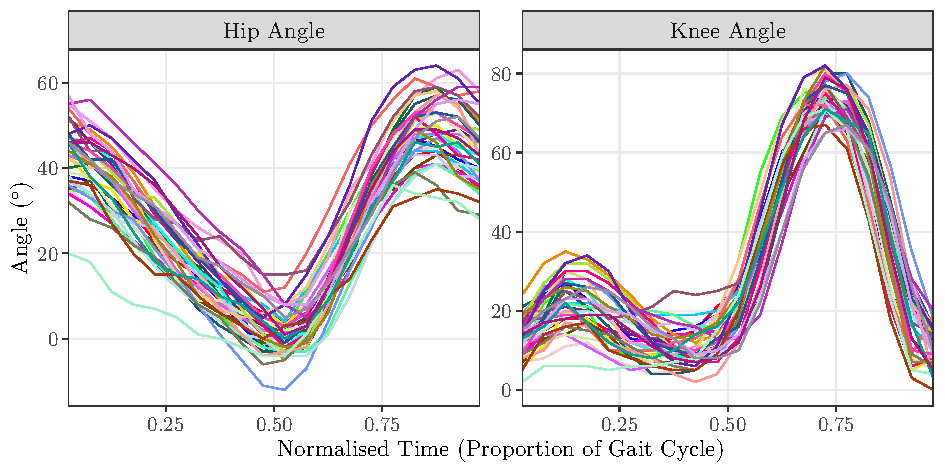
\includegraphics[width=0.5\textwidth, page = 1]{figures/thesis-chapt-1-2.pdf}
    \caption{The childrens' gait dataset \parencite{rice_estimating_1991}.}
    \label{fig:enter-label}
\end{figure}
\end{frame}

\begin{frame}{Second-Generation Functional Data in Biomechanics}
    \begin{columns}[c] % The "c" option specifies centered vertical alignment while the "t" option is used for top vertical alignment
        \centering
        \column{.33\textwidth} % Left column and width
        \centering
        \textbf{Volume} 
        \vskip1em
        \centering
        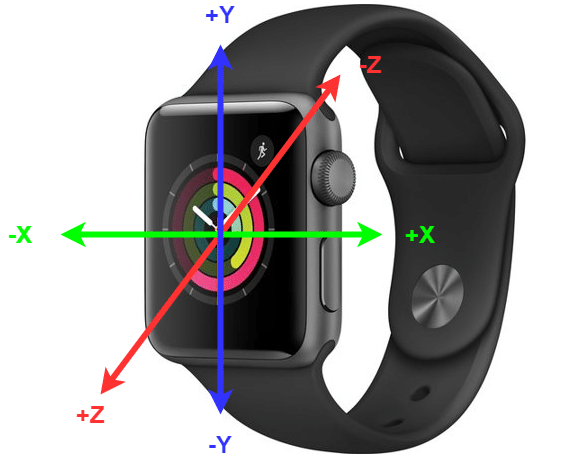
\includegraphics[width = 0.4 \textwidth]{figures/Apple-watch-series-1-used-for-recording-accelerometer-and-gyroscope-signals.png}
        \vskip1em
        \centering
        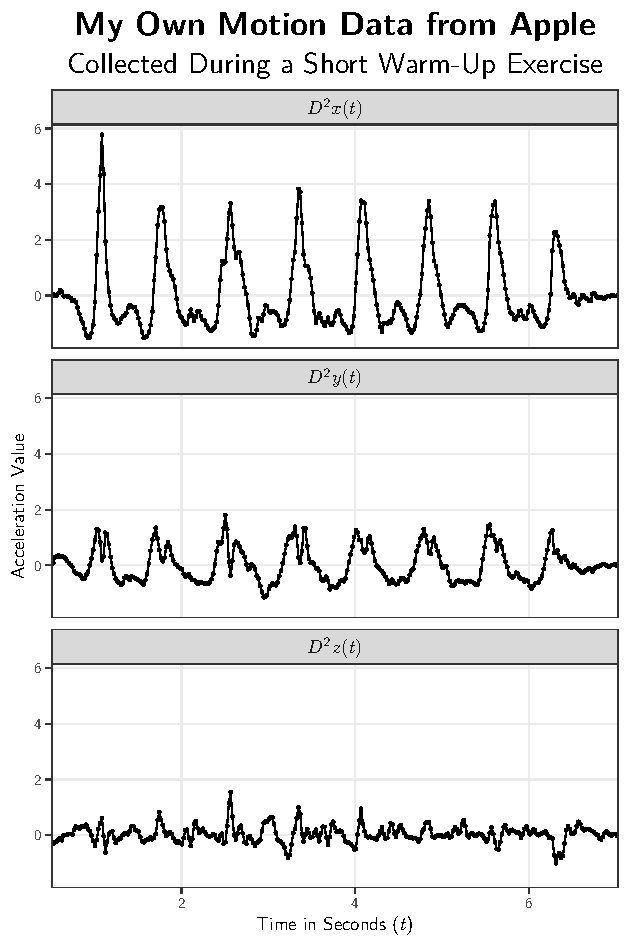
\includegraphics[width = 0.75\textwidth]{figures/my-apple-data.pdf}

        \pause \column{.33\textwidth} % Right column and width
        \centering
        \textbf{Complexity}
        \vskip1em
        \vfill
        \centering 
        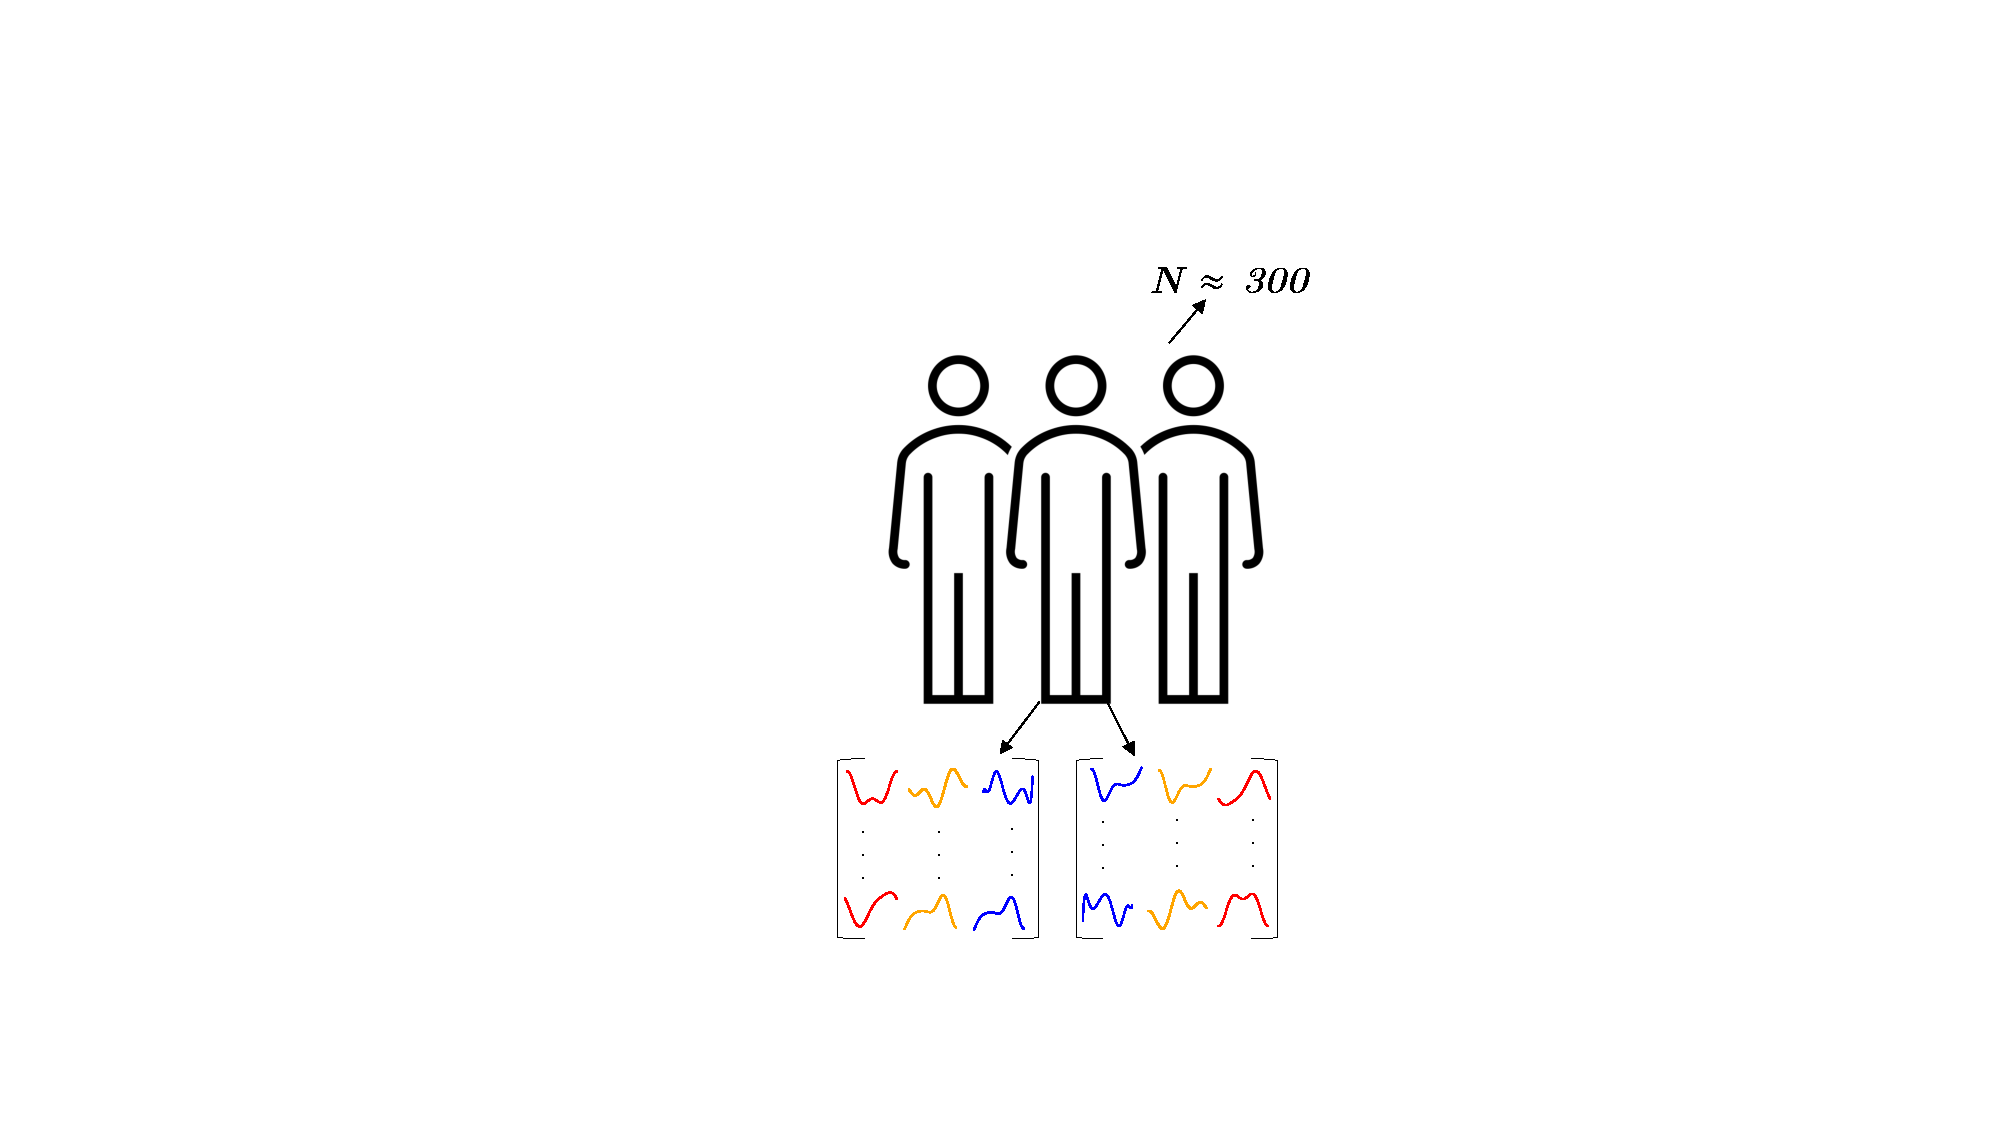
\includegraphics[width = 0.7\textwidth]{figures/Multilevel-Data-Figure.pdf}
        \vskip1em
        \centering
        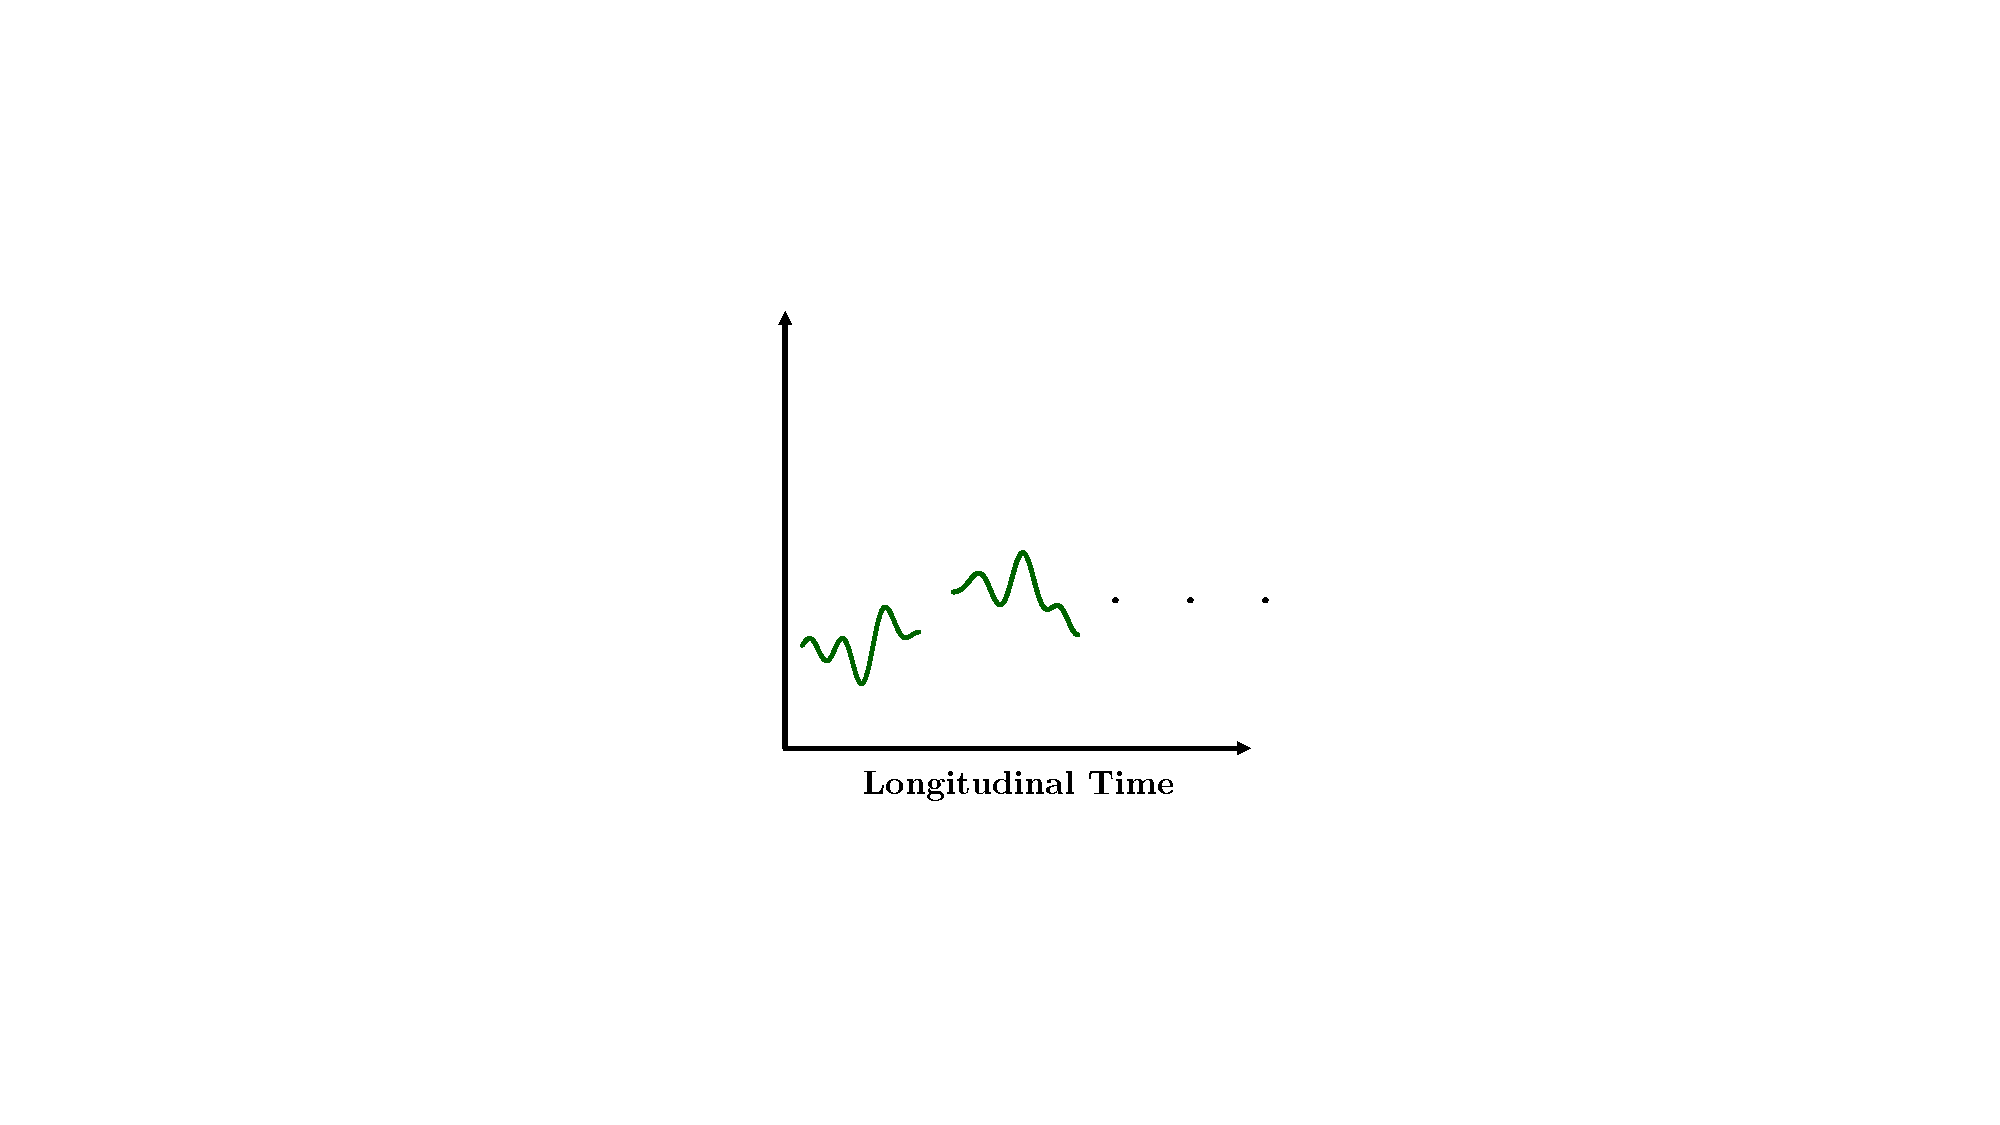
\includegraphics[width = 0.6\textwidth]{figures/Longitudinal-Figure.pdf}

        
        \pause \column{.33\textwidth} % Right column and width
        \centering
        \textbf{Variety}
        \vskip2em
        \centering
        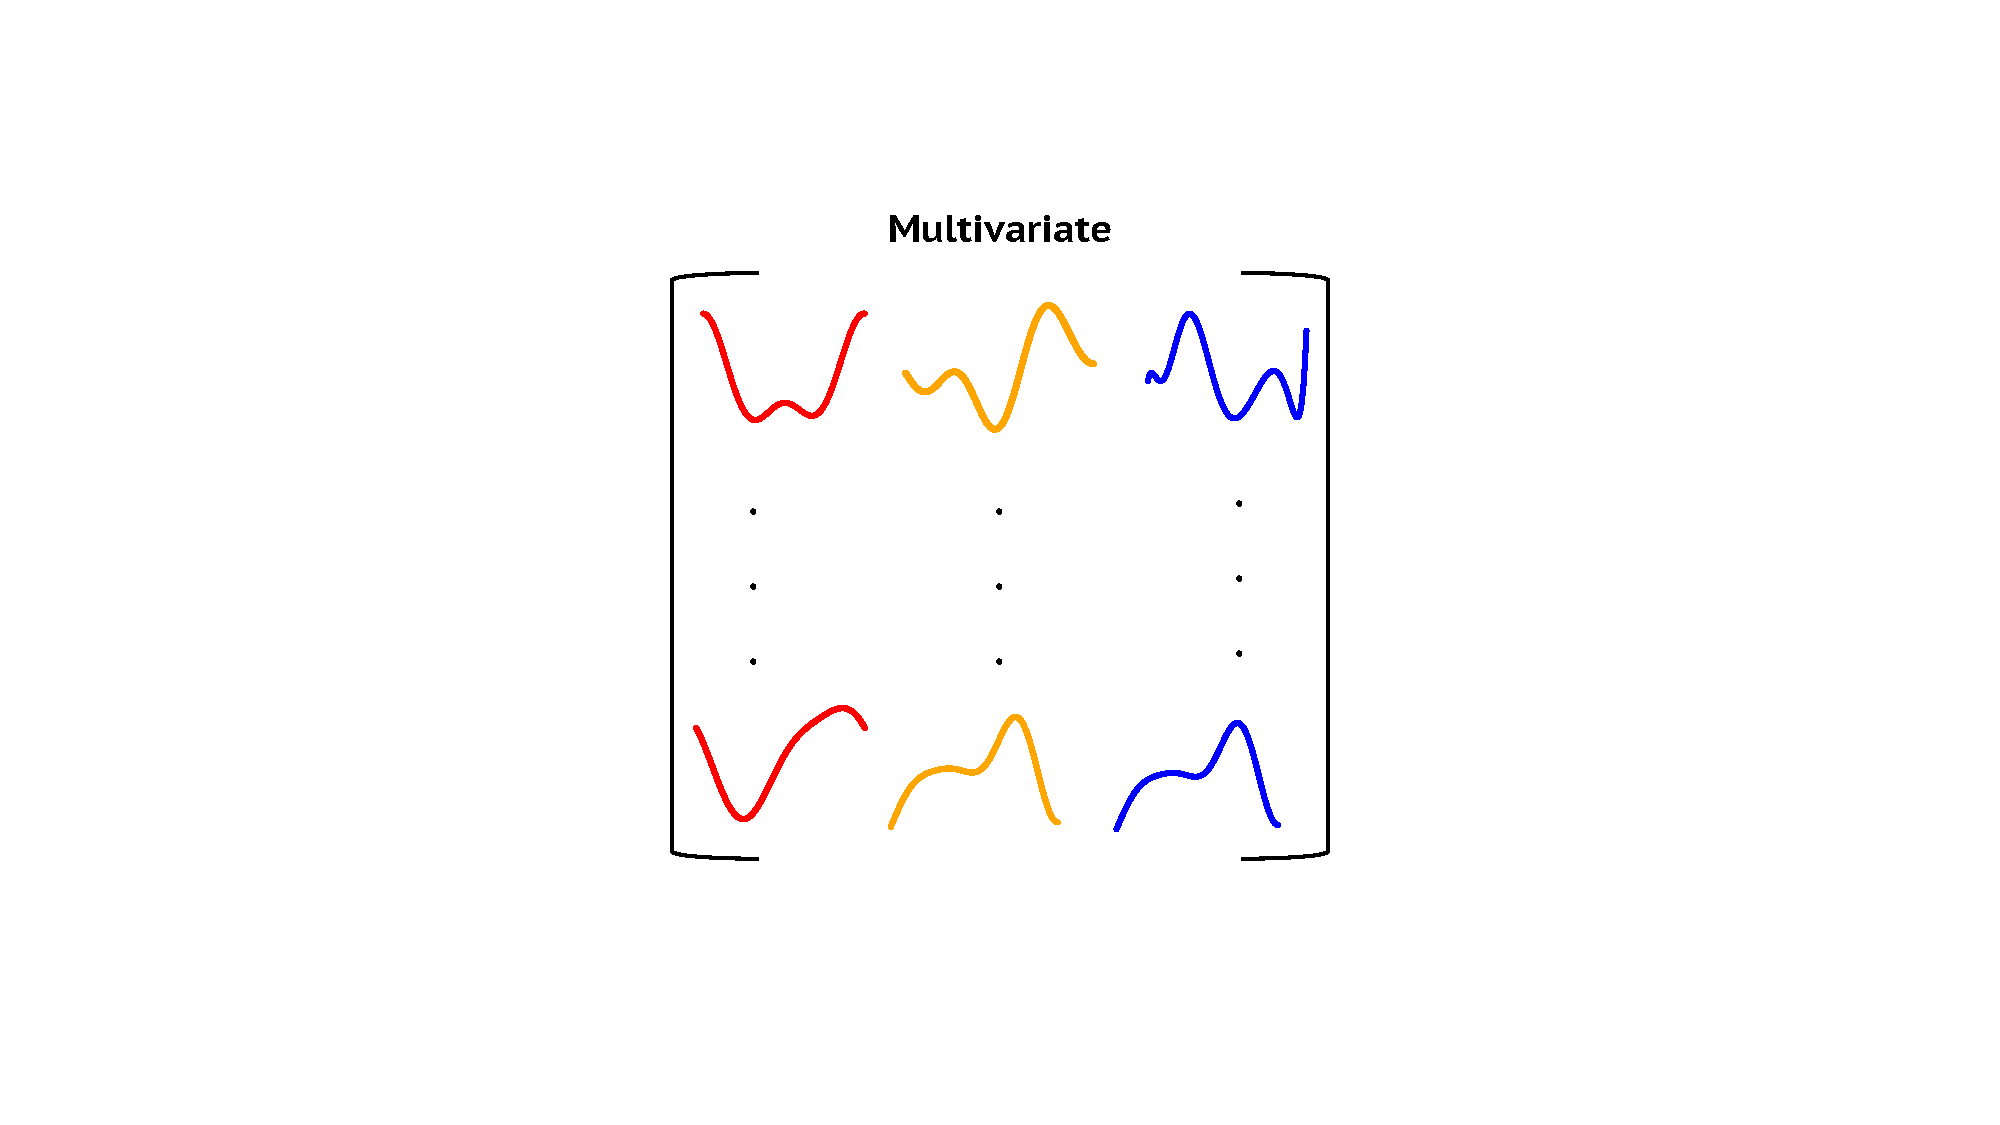
\includegraphics[width = 0.75\textwidth]{figures/Multivariate.pdf}
        \vskip1em
        Human movement as a system of multiple related parts $\rightarrow$ \textbf{multivariate} and \textbf{dynamical systems} approaches to analysis.
    \end{columns}
\end{frame}








% End


\begin{frame}{More Information}
\small
   \textbf{Literature}:
   \begin{itemize}
       \item \fullcite{gunning_analyzing_2023}
       \item \fullcite{gunning_multivariate_2023}
       \item \fullcite{gunning_understanding_2023}
   \end{itemize}
\textbf{Email}: \href{mailto:edward.gunning@pennmedicine.upenn.edu}{edward.gunning@pennmedicine.upenn.edu}

%%% Intro


\textbf{Website}: \url{https://edwardgunning.github.io/}

   
   \textbf{\href{https://link.springer.com/book/9783031688614}{Upcoming Book}}:
   \begin{figure}
       \centering
       
\includegraphics[width=0.125\linewidth]{figures/book_frontcover.png}
       % \caption{Caption}
       % \href{https://link.springer.com/book/9783031688614}{\emph{\small Functional Data Analysis in Biomechanics: A Concise Review of Core Techniques, Applications and Emerging Areas}}
       \label{fig:enter-label}
   \end{figure}
\end{frame}

%----------------------------------------------------------------------------------------


\begin{frame}[noframenumbering]{References}
       \printbibliography
\end{frame}

\end{document}